The goal of this section is to present the overall proof strategy that
we adopted to establish the semantic preservation property for the
\hilecop{} model-to-text transformation. We take advantage of the
proof of Lemma~\ref{lem:fe-equal-fired}, involved in the proof of
Lemma~\ref{lem:fe}, to illustrate our demonstration techniques. The
proof of Lemma~\ref{lem:fe-equal-fired} has been one complex part of
the overall demonstration; we believe it is worth to be
mentioned. Also, it has led to a bug detection. We give a full account
on this bug detection, and on how we manage to correct it, at the end
of the section.

\subsection{An accompanied journey along the proof}
\label{sec:informal-fired-proof}

The proof of Lemma~\ref{lem:fe-equal-fired} is related to the set of
fired transitions. In an SITPN, the firing process, based on the set
of fired transitions, is responsible for the computation of the new
marking, the reset orders, and the execution of functions during the
rising edge phase. To prove the semantic preservation property, we
must have the equivalence between the set of fired transitions as
defined on the SITPN side and the set of fired transitions as defined
on the \hvhdl{} side. The equivalence must hold at the beginning of
the rising edge phase, i.e. when the set of fired transitions will be
used to compute a new SITPN state. Thus, the falling edge phase
prepares the ground so that the equivalence between the set of fired
transitions holds at the beginning of the next rising edge phase. To
express Lemma~\ref{lem:fe-equal-fired}, we must first define the
hypotheses stating that a falling edge phase happened in the course of
the execution of an SITPN and its corresponding \hvhdl{} design, plus
some hypotheses about the similarity of the states at the beginning of
the falling edge phase:

%%%%%%%%%%%%%%%%%%%%%%%%%%%%%%%%%%%%%%%%%%%%% 
%%%%%%%%%% FALLING EDGE HYPOTHESES %%%%%%%%%%
%%%%%%%%%%%%%%%%%%%%%%%%%%%%%%%%%%%%%%%%%%%%%

\begin{definition}[Falling edge hypotheses]
  \label{def:fe-hyps}
  Given a $sitpn\in{}SITPN$, $b\in{}P\rightarrow\mathbb{N}$,
  $d\in{}design$, $\gamma\in{}WM(sitpn,d)$,
  $E_c\in\mathbb{N}\rightarrow\mathcal{C}\rightarrow\mathbb{B}$,
  $\Delta\in{}ElDesign$,
  $E_p\in\mathbb{N}\rightarrow{}Ins(\Delta)\rightarrow{}value$,
  $\tau\in\mathbb{N}$, $s,s'\in{}S(sitpn)$,
  $\sigma_e,\sigma,\sigma_\downarrow,\sigma'\in\Sigma$, assume that:
  \begin{itemize}
  \item SITPN $sitpn$ is transformed into the \hvhdl{} design $d$ and
    yields the binder $\gamma$: $\lfloor{}sitpn\rfloor_b=(d,\gamma)$
  \item Simulation/Execution environments are similar:
    $\gamma\vdash{}E_p\stackrel{env}{=}E_c$
  \item $\Delta$ is the elaborated version of design $d$, and
    $\sigma_e$ is the default design state of $\Delta$:
    $\mathcal{D}_\mathcal{H},\emptyset\vdash\mathrm{d}\srarrow{elab}{\fontsize{5}{7}\selectfont}\Delta,\sigma_e$
  \item Starting states are similar according to the full post rising
    edge similarity relation:
    $\gamma,E_c,\tau\vdash{}s\stackrel{\uparrow}{\approx}\sigma$
  \item On the SITPN side, the execution of a falling edge phase
    starting from state $s$ leads to state $s'$:\\
    $E_c,\tau\vdash{}s\xrightarrow{\downarrow}s'$
  \item On the \hvhdl{} side, the simulation of a falling edge phase
    starting from state $\sigma$ leads to state $\sigma'$:
    $\Delta,\sigma\vdash\mathrm{d.cs}\xrightarrow{\downarrow}\sigma_{\downarrow}$
    and
    $\Delta,\sigma_{\downarrow}\vdash\mathrm{d.cs}\xrightarrow{\rightsquigarrow}\sigma'$
  \item State $\sigma$ is a stable design state:
    $\mathcal{D}_{\mathcal{H}},\Delta,\sigma\vdash\mathrm{d.cs}\xrightarrow{comb}\sigma$
  \end{itemize}
\end{definition}

\def\fehyps{For all $sitpn$, $b$, $d$, $\gamma$, $\Delta$, $\sigma_e$,
  $E_c$, $E_p$, $\tau$, $s$, $s'$, $\sigma$, $\sigma_{\downarrow}$,
  $\sigma'$ that verify the hypotheses of
  Definition~\ref{def:fe-hyps},}

The hypotheses of Definition~\ref{def:fe-hyps} are used in all the
lemmas expressing properties of the falling edge phase. Therefore,
Definition~\ref{def:fe-hyps} enables the conciser expression of these
lemmas. Then, we can express Lemma~\ref{lem:fe-equal-fired} as
follows:

\begin{lemma}[Falling edge equal fired]
  \label{lem:fe-equal-fired}
  \fehyps{} then for all
  $t\in{}T,id_t\in{}Comps(\Delta)~s.t.~\gamma(t)=id_t,$
  $t\in{}Fired(s')\Leftrightarrow\sigma'(id_t)(\texttt{fired})=\mathtt{true}$.
\end{lemma}

Now, let us detail the proof of Lemma~\ref{lem:fe-equal-fired}. To
prove Lemma~\ref{lem:fe-equal-fired}, we must reason on a given
transition $t$ of the input SITPN $sitpn$ and a TCI $id_t$ in the
output \hvhdl{} design $d$. Transition $t$ and TCI $id_t$ are bound
together through the $\gamma$ binder returned by the transformation
function. This means that the TCI $id_t$ structurally represents the
transition $t$ in the output \hvhdl{} design $d$. In this setting, we
want to prove that $t$ is in the set of fired transitions at the end
of the falling edge phase if and only if the \texttt{fired} port of
$id_t$ equals $\mathtt{true}$ at the end of the falling edge
phase. Formally, we want to prove:
\fbox{$t\in{}Fired(s')\Leftrightarrow\sigma'(id_t)(\texttt{fired})=\mathtt{true}$.}

As a reminder, the expression $Fired(s')$ qualifies the set of fired
transitions at the SITPN state $s'$, and
$\sigma'(id_t)(\texttt{fired})$ denotes the value of the
\texttt{fired} port of TCI $id_t$ at design state $\sigma'$. The
expression $\sigma'(id_t)$ denotes the internal state, i.e. a design
state, of TCI $id_t$ at state $\sigma'$.

To prove the equivalence, we must first look at the definition of the
set of fired transitions on the SITPN side and on the \hvhdl{} side,
and then think of a way to relate the two definitions.

On the SITPN side, the set of fired transitions is an intentional and
recursive definition (see Definition~\ref{def:fired}) depending on a
given SITPN state. In Lemma~\ref{lem:fe-equal-fired}, we are
interested in the definition of the set of fired transitions at state
$s'$, i.e. the state at the end of the falling edge phase. A
transition belongs to the set of fired transitions if it is
\emph{firable} (see Definition~\ref{def:firable}) and sensitized by
the \emph{residual} marking (see
Sections~\ref{subsec:hpn-particularities} and \ref{sec:fired-trans})
at the considered SITPN state.  Figure~\ref{fig:example-fired-trans}
gives the set of fired transitions, i.e. $Fired(s)$, on an example of
SITPN at a given state $s$. Here, transitions $t_a$, $t_b$ and $t_c$
are all firable at state $s$; however, only transition $t_c$ is
sensitized by the residual marking.

\begin{figure}[H]
  \centering
  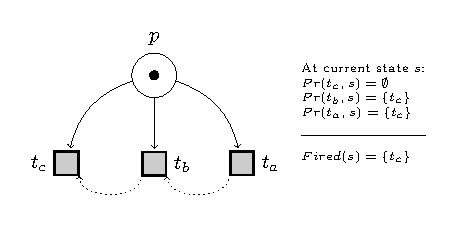
\includegraphics[keepaspectratio,width=.6\textwidth]{Figures/Proof/example-fired-trans}
  \caption[A set of fired transitions.]{The set of fired transitions
    on an example SITPN at a given SITPN state $s$; on the left side,
    the dotted arrows indicates the priority relation between the
    three transitions ($t_c$ is the top-priority transition); on the
    right side, each transition is associated to its $Pr$ set, which
    is necessary to compute the residual marking.  }
  \label{fig:example-fired-trans}
\end{figure}

The computation of the residual marking involves the $Pr$ sets, which
are, for a given transition $t$ and a state $s$, the set of
transitions with a higher firing priority than $t$ which are actually
fired at $s$. This is where the recursive definition of the set of
fired transitions begins. The definition is correct, i.e. the
recursion ends, if the priority relation is a strict order over the
set of transitions, and therefore, there are always transitions of
top-priority (e.g, $t_c$ in Figure~\ref{fig:example-fired-trans}). The
condition of the priority relation being a strict order over the set
of transitions is part of the definition of a well-defined SITPN (see
Definition~\ref{def:wd-sitpn}). By definition, top-priority
transitions have an empty $Pr$ set. There exists no transition with a
higher firing priority than a top-priority transition. Thus, a
top-priority transition that is firable is also fired. Note that one
cannot determine the $Pr$ set of a transition before having determined
the firing status of all the transitions with a higher firing
priority. For instance, in Figure~\ref{fig:example-fired-trans}, it is
impossible to know the content of $Pr(t_a,s)$ before having determined
if transition $t_b$ is fired or not. To know if $t_b$ is fired or not,
we must determine the content of $Pr(t_b,s)$. To do so, we must first
determine the firing status of $t_c$. Even though the definition of
the set of fired transitions is very declarative, this provides a
natural way to establish an algorithm to build the set of fired
transitions at a given SITPN state.

On the \hvhdl{} side, the set of fired transitions is defined through
the value of the \texttt{fired} port of TCIs. The transition design
declares an output port of the Boolean type with the identifier
\texttt{fired}. What we want to prove in
Lemma~\ref{lem:fe-equal-fired} is that, at the end of the falling edge
phase (i.e. at state $\sigma'$), the value of the \texttt{fired} port
of a TCI reflects the firing status of the corresponding
transition. The \texttt{fired} port is a combinational signal. This
means that its value depends on an equation that is verified when all
signals are stable, i.e. at the end of stabilization phases happening
during the simulation. In the point of view of the circuit synthesis,
this equation reflects the wiring of the port in the described
hardware circuit. Figure~\ref{fig:fired-port} shows a part of the
transition design architecture describing how the \texttt{fired} port
is connected to the other internal signals.

\begin{figure}[H]
  \centering
  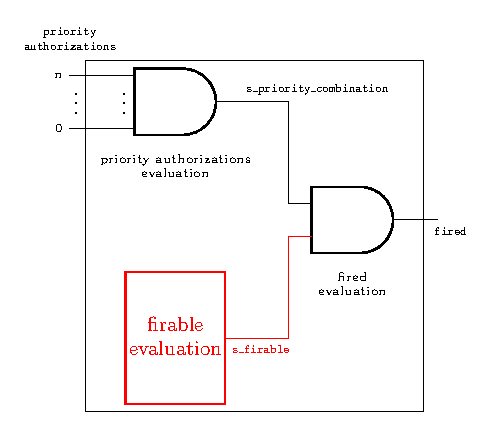
\includegraphics[keepaspectratio, width=.6\textwidth]{Figures/Proof/fired-port}
  \caption[The \texttt{fired} output port in the transition design
  architecture.]{Wiring of the \texttt{fired} output port in the
    transition design architecture; on the left side is the input
    interface of the transition design; on the right side is the
    output interface of the transition design, with the \texttt{fired}
    port; in red are the parts of the architecture that depend on
    synchronous logic and in black are the parts that are purely
    combinational.}
  \label{fig:fired-port}
\end{figure}

In Figure~\ref{fig:fired-port}, the labels underneath the \emph{and}
logic ports and inside the block denote the names of the processes
defined in the transition design architecture as \vhdl{} code. As a
matter of fact, Figure~\ref{fig:fired-port} is a graphical
transcription of the code defining the transition design
architecture. Therefore, by looking at the \vhdl{} code, we are able
to determine the combinational equation associated to the
\texttt{fired} port. Given a TCI $id_t$ in a top-level design and a
state $\sigma$ denoting a current stable state of the design (remember
that a combinational equation holds when all signal values are
stable), the \texttt{fired} port equation at $\sigma$ is:

\begin{equation}
  \label{eq:fired-port-comb-eq}
  \sigma(id_t)(\texttt{fired})=\sigma(id_t)(\texttt{s\_firable})~.~\sigma(id_t)(\texttt{s\_priority\_combination})
\end{equation}

Equation~\eqref{eq:fired-port-comb-eq} states that the value of the
\texttt{fired} port is a simple ``and'' expression\footnote{To
  differentiate the formulas of the first-order logic from the
  expressions of the Boolean logic, we use (``$.$'', ``+'') to denote
  the \emph{and} and \emph{or} operators in Boolean expressions, and
  ($\land$,$\lor$) to denote the conjunction and the disjunction in
  the first-order logic formulas.} between the value of the internal
signal \texttt{s\_firable} and \texttt{s\_priority\_combination}.

\begin{remark}[Signals and combinational equations]
  \label{rmk:comb-eqs}
  In the proceeding of the proof, a lot of combinational equations are
  established (e.g, Equation~\eqref{eq:fired-port-comb-eq}). These
  equations relate the value of a given signal to the value of other
  signals or expressions. All these equations are deduced by applying
  the \hvhdl{} semantics rules on the internal behavior (i.e., the
  processes) of the \texttt{transition} and the \texttt{place}
  designs. A combinational equation is always the result of a signal
  assignment statement happening inside the statement body of a
  process. For instance, in the transition design, the
  \texttt{fired\_evaluation} process, presented in
  Listing~\ref{lst:fired-eval-ps}, assigns the \texttt{fired} output
  port.  Reasoning on the \texttt{fired\_evaluation} process statement
  body and on the \hvhdl{} semantics rules permits us to deduce
  Equation~\eqref{eq:fired-port-comb-eq}.

\begin{lstlisting}[language=VHDL,label={lst:fired-eval-ps},caption={The \texttt{fired\_evaluation} process in the transition design architecture; its statement body assigns the \texttt{fired} output port; symbol $\Leftarrow$ is the signal assignment operator}.]
fired_evaluation : process (s_firable, s_priority_combination)
begin
   fired <= s_firable and s_priority_combination;
end process fired_evaluation;
\end{lstlisting}

  Listing~\ref{lst:pauths-eval-ps} presents the
  \texttt{priority\_}\texttt{authorizations\_}\texttt{evaluation}
  process, responsible for the assignment of the
  \texttt{s\_priority\_combination} in the transition
  design. 

\begin{lstlisting}[language=VHDL,label={lst:pauths-eval-ps},caption={The \texttt{priority\_authorizations\_evaluation} process in the transition design's architecture. The local variable \texttt{v\_priority\_combination} accumulates the product of the subelements of the \texttt{priority\_authorizations} input port in the \texttt{for} loop; then the last statement assigns the value of \texttt{v\_priority\_combination} to the \texttt{s\_priority\_combination} internal signal.}]
priority_authorization_evaluation : process(priority_authorizations)
   variable v_priority_combination : std_logic;
begin
   v_priority_combination := '1';
    
   for i in 0 to input_arcs_number $-$ 1 loop
     v_priority_combination := v_priority_combination and priority_authorizations(i);
   end loop;
    
   s_priority_combination <= v_priority_combination; -- Assignment of the result
end process priority_authorization_evaluation;
\end{lstlisting}

  Equation~\eqref{eq:spc-comb-eq} gives the combinational equation
  deduced from the execution of the
  \texttt{priority\_}\texttt{authorizations\_}\texttt{evaluation}
  process for a given TCI $id_t$ in a top-level design $d$. State
  $\sigma$ denotes the current state of $d$, and $\sigma(id_t)$
  denotes the internal state of $id_t$ at state $\sigma$. The
  elaborated design $\Delta$ is the elaborated version of design $d$,
  and $\Delta(id_t)$ is the elaborated version of $id_t$.
  
  \begin{equation}
    \label{eq:spc-comb-eq}
    \sigma(id_t)(\texttt{spc})=\prod\limits_{i=0}^{\Delta(id_t)(\texttt{input\_arcs\_number})-1}\sigma(id_t)(\texttt{priority\_authorizations})[i]
  \end{equation}

  In Equation~\eqref{eq:spc-comb-eq}, \texttt{spc} is an alias for the
  \texttt{s\_priority\_combination} signal.  The \texttt{for} loop of
  the \texttt{priority\_authorization\_evaluation} process has been
  converted into a product expression where the index $i$ follows the
  bounds of the loop. The \texttt{priority\_authorizations} signal is
  an input port of type \texttt{array}, thus we use the bracketed
  notation $a[i]$ to access the element of index $i$ in array
  $a$. Also, we know that \texttt{input\_arcs\_number} identifies a
  generic constant of the transition design, thus, we can retrieve its
  value in the elaborated design $\Delta(id_t)$.
  
  In the proofs laid out in Appendix~\ref{app:sem-preserv-proof} and
  in this chapter, we do not detail how the execution of processes'
  statement body permit to deduce combinational equations. We find
  that the proofs are easier to follow without entering in so much
  details. We let aside the task of proving that these equations hold
  until the time of the mechanization with the \coq{} proof
  assistant. For now, the reader can convince himself/herself that an
  equation holds by looking at the code of the \texttt{place} and the
  \texttt{transition} designs (see Appendices~\ref{app:place-design}
  and \ref{app:trans-design}).
\end{remark}

Now that we know which combinational equation is attached to the value
of the output port \texttt{fired} for a given TCI, we must relate this
equation to the definition of the set of fired transitions on the
SITPN side. By definition of the set of fired transitions, we know
that $t\in{}Fired(s')$ is equivalent to
$t\in{}Firable(s')\land{}t\in{}Sens(s'.M-\sum\limits_{t_i\in{}Pr(t,s')}pre(t_i))$
where $Pr(t,s')=\{t'~\vert~t'\succ{}t\land{}t'\in{}Fired(s')\}$. By
definition of the \texttt{fired} port equation, we know that
$\sigma'(id_t)(\texttt{fired})=\sigma'(id_t)(\texttt{s\_firable})~.~\sigma'(id_t)(\texttt{s\_priority\_combination})$.
Using these definitions to rewrite the terms of the current goal, the
new goal to prove is:

\begin{frameb}
  $t\in{}Firable(s')\land{}t\in{}Sens(s'.M-\sum\limits_{t_i\in{}Pr(t,s')}pre(t_i))\Leftrightarrow$\\
  $\sigma'(id_t)(\texttt{s\_firable})~.~\sigma'(id_t)(\texttt{s\_priority\_combination})=\mathtt{true}$
\end{frameb}

Thanks to Lemma~\ref{lem:fe-equal-firable}, we know that
$t\in{}Firable(s')$ iff
$\sigma'(id_t)(\texttt{s\_firable})=\mathtt{true}$. Then, we can get
rid of these two terms in the current goal; what is left to prove is:

\begin{frameb}
  $t\in{}Sens(s'.M-\sum\limits_{t_i\in{}Pr(t,s')}pre(t_i))\Leftrightarrow$
  $\sigma'(id_t)(\texttt{s\_priority\_combination})=\mathtt{true}$
\end{frameb}

Based on Equation~\eqref{eq:spc-comb-eq}, we can replace the value of
the \texttt{s_priority_combination} signal by its equivalent product
expression:

\begin{frameb}
  $t\in{}Sens(s'.M-\sum\limits_{t_i\in{}Pr(t,s')}pre(t_i))\Leftrightarrow$\\
  $\big(\prod\limits_{i=0}^{\Delta(id_t)(\texttt{input\_arcs\_number})-1}\sigma'(id_t)(\texttt{priority\_authorizations})[i]\big)=\mathtt{true}$
\end{frameb}

\noindent{}Then, the proof is in two parts:

\begin{enumerate}
\item Assuming
  $t\in{}Sens(s'.M-\sum\limits_{t_i\in{}Pr(t,s')}pre(t_i))$, let us
  show that\\
  \fbox{$\big(\prod\limits_{i=0}^{\Delta(id_t)(\texttt{ian})-1}\sigma'(id_t)(\texttt{pauths})[i]\big)=\mathtt{true}$.}
\item Assuming
  $\big(\prod\limits_{i=0}^{\Delta(id_t)(\texttt{ian})-1}\sigma'(id_t)(\texttt{pauths})[i]\big)=\mathtt{true}$,
  let us show that\\
  \fbox{$t\in{}Sens(s'.M-\sum\limits_{t_i\in{}Pr(t,s')}pre(t_i))$.}
\end{enumerate}

\noindent{}Let us prove the first point. Assuming that
$t\in{}Sens(s'.M-\sum\limits_{t_i\in{}Pr(t,s')}pre(t_i))$, let us
show\\
\fbox{$\big(\prod\limits_{i=0}^{\Delta(id_t)(\texttt{ian})-1}\sigma'(id_t)(\texttt{pauths})[i]\big)=\mathtt{true}$.}\\

\noindent{}To prove the current goal, we can equivalently show that:\\
\fbox{$\forall{}i\in[0,\Delta(id_t)(\texttt{ian})-1],~\sigma'(id_t)(\texttt{pauths})[i]=\mathtt{true}$.}\\

\noindent{}For a given $i\in[0,\Delta(id_t)(\texttt{ian})-1]$, let us
show that \fbox{$\sigma'(id_t)(\texttt{pauths})[i]=\mathtt{true}$.} As
shown in Figure~\ref{fig:fired-port}, the
\texttt{priority\_authorizations} signal is an input port of the
\texttt{transition} design. Therefore, to know what is the value of
the $i$-th element of the \texttt{priority\_authorizations} port at
state $\sigma'(id_t)$, we must know how the
\texttt{priority\_authorizations} port is connected in the top-level
design. Basing ourselves on the transformation function
(cf. Algorithm~\ref{alg:geninter}, p.~\pageref{alg:geninter}), the
connection of the \texttt{priority\_authorizations} port for the TCI
$id_t$ depends on the set of input places of the transition $t$. If
the set of input places of $t$ is empty, then, all elements of the
\texttt{priority\_authorizations} port are connected to the constant
\texttt{true}, and proving the goal is trivial. If the set of input
places of $t$ is not empty, then, the connection of the $i$-th element
of the \texttt{priority\_authorizations} port reflects the connection
of some place $p$ to the transition $t$ by an input arc. Then, we must
reason on the nature of the input arc connecting $p$ to $t$. The
interested case happens when $p$ and $t$ are connected by a
\texttt{basic} arc, and when the conflicts in the output transitions
of $p$ are handled by the priority relation. In that case, the $i$-th
element of the \texttt{priority\_authorizations} input port of the TCI
$id_t$ is connected to the $j$-th element of the
\texttt{priority\_authorizations} output port of the PCI
$id_p$. Figure~\ref{fig:pauths-connection} shows the connection of the
\texttt{priority\_authorizations} port between the component instances
$id_p$ and $id_t$.

\begin{figure}[H]
  \centering
  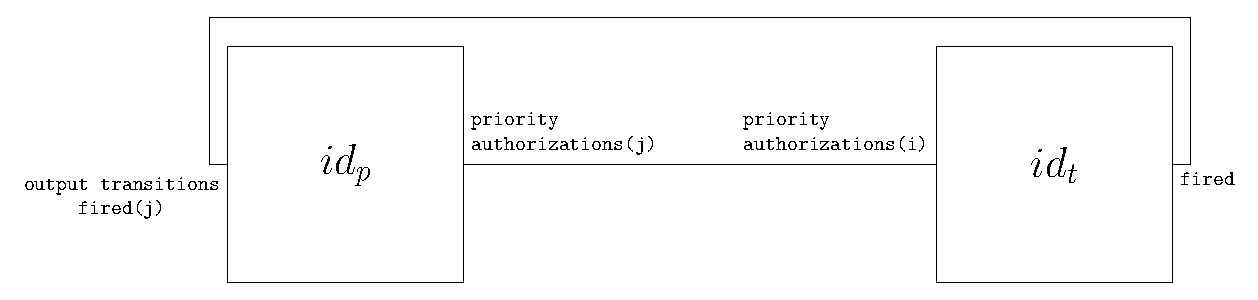
\includegraphics[keepaspectratio, width=.8\textwidth]{Figures/Proof/pauths-connection}
  \caption[Connection of the \texttt{priority\_authorizations} ports
  and of the \texttt{fired} and \texttt{output\_transitions\_fired}
  ports between a PCI and a TCI.]{Connection of the $j$-th element of
    the \texttt{priority\_authorizations} output port of the PCI
    $id_p$ to the $i$-th element of the
    \texttt{priority\_authorizations} input port of the TCI $id_t$;
    also the \texttt{fired} output port of $id_t$ is connected to the
    $j$-th element of the \texttt{output\_transitions\_fired} input
    port of $id_p$.}
  \label{fig:pauths-connection}
\end{figure}

Thus, we know that the value of the $i$-th element of the
\texttt{priority\_authorizations} input port of $id_t$ is bound to the
value of the $j$-th element of the \texttt{priority\_authorizations}
output port of $id_p$. Therefore, to show that
\fbox{$\sigma'(id_t)(\texttt{pauths})[i]=\mathtt{true}$}, we must now
show that \fbox{$\sigma'(id_p)(\texttt{pauths})[j]=\mathtt{true}$.} We
must now look at the architecture of the \texttt{place} design to
determine the combinational equation associated to the $j$-th element
of the \texttt{priority\_authorizations} output
port. Figure~\ref{fig:pauths-in-p} illustrates the wiring of the
\texttt{priority\_authorizations} output port in a \texttt{place}
design.

\begin{figure}[H]
  \centering
  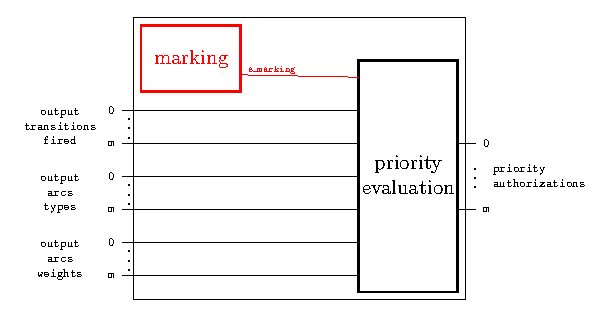
\includegraphics[keepaspectratio,width=.7\textwidth]{Figures/Proof/pauths}
  \caption[The \texttt{priority\_authorizations} output port
  in the place design architecture.]{Wiring of the
    \texttt{priority\_authorizations} output port in the architecture
    of the place design; the input port interface is on the left side
    and the output port interface is on the right side; the
    synchronous parts are in red and the combinational ones are in
    black.}
  \label{fig:pauths-in-p}
\end{figure}

Figure~\ref{fig:pauths-in-p} shows that the value of the elements of
the \texttt{priority\_authorizations} output port is computed by the
\texttt{priority\_evaluation} process. This process reads the value of
the \texttt{s\_marking} signal, assigned by the synchronous process
\texttt{marking}. It also reads the value of the
\texttt{output\_transitions\_fired}, \texttt{output\_arcs\_types} and
\texttt{output\_arcs\_weights} input ports.  In
Figure~\ref{fig:pauths-in-p}, the ports of the input and output
interface are composite ports (i.e., of the array type) with an upper
bound index equal to \texttt{m}. The number $\mathtt{m}$ is equal to
the expression \texttt{output\_arcs\_number}$-1$, where
\texttt{output\_arcs\_number} is a generic constant of the place
design. The value of the \texttt{output\_arcs\_number} constant is set
at the generation of the generic map of a PCI $id_p$, and is equal to
the number of output transitions of place
$p$. Listing~\ref{lst:pauths-out-eval-ps} presents the code of the
\texttt{priority\_evaluation} process defined in the architecture of
the \texttt{place} design.

\begin{lstlisting}[language=VHDL,label={lst:pauths-out-eval-ps},caption={The \texttt{priority\_evaluation} process in the place design's architecture.},framexleftmargin=1.5em,xleftmargin=2em,numbers=left, numberstyle=\tiny\ttfamily]
priority_evaluation : process (output_transitions_fired, s_marking, output_arcs_types, output_arcs_weights)
  variable v_saved_output_token_sum : local_weight_t;
begin
  v_saved_output_token_sum := 0;
    
  for k in 0 to output_arcs_number $-$ 1 loop

    priority_authorizations(k) <= (s_marking $-$ v_saved_output_token_sum >= output_arcs_weights(k));
      
    if (output_transitions_fired(k) = '1') and (output_arcs_types(k) = arc_t(BASIC)) then
      v_saved_output_token_sum := v_saved_output_token_sum + output_arcs_weights(k);
    end if;
      
  end loop;
end process priority_evaluation;
\end{lstlisting}

In the statement body of the \texttt{priority\_evaluation} process,
each subelement of the \texttt{priority\_authorizations} output port is
assigned at Line~8 inside the \texttt{for} loop. The statement of Line~8
assigns the result of the test \texttt{s_marking $-$ v_saved_output_token_sum >= output_arcs_weights(k)} to the $k$-th
element of \vhdle|priority_authorizations|.  The test checks that the
value of the \texttt{s\_marking} signal, representing the current
marking of the PCI, minus the value of the local variable
\texttt{v\_saved\_output\_token} is greater than or equal to the value
of the $k$-th element of the \texttt{output\_arcs\_weights}
signal. The test corresponds to the test of sensitization by the
residual marking for the TCI connected through index $k$.

Getting back to our proof, the following combinational equation holds
for the $j$-th element of the \texttt{priority\_authorizations} port
at state $\sigma'$:
\begin{equation}
  \label{eq:pauths-j-comb-eq}
  \sigma'(id_p)(\texttt{pauths})[j]=(\sigma'(id_p)(\texttt{s\_marking})-\mathtt{vsots}\ge\sigma'(id)(\texttt{output\_arcs\_weights})[j])
\end{equation}

\noindent{}Then, rewriting the goal with Equation~\eqref{eq:pauths-j-comb-eq},
the new goal is:\\
\fbox{$(\sigma'(id_p)(\texttt{s\_marking})-\mathtt{vsots}\ge\sigma'(id)(\texttt{output\_arcs\_weights})[j])=\mathtt{true}$.}\\

Here $\ge$ denotes a Boolean operator, i.e.
$\ge\in\mathbb{N}\rightarrow\mathbb{N}\rightarrow\mathbb{B}$. As the
$\ge\subseteq{}(\mathbb{N}\times\mathbb{N})$ relation is decidable for
all pairs of natural numbers, we can interchange an expression
$a\ge{}b=\mathtt{true}$ with $a\ge{}b$ where $a,b\in\mathbb{N}$. We
will generalize this practice to every Boolean operator having a
corresponding decidable relation. Thus, the new goal is:\\
\fbox{$\sigma'(id_p)(\texttt{s\_marking})-\mathtt{vsots}\ge\sigma'(id)(\texttt{output\_arcs\_weights})[j]$.}\\

Here, the term $\mathtt{vsots}$ corresponds to the value of the local
variable \texttt{v\_saved\_output\_token\_sum} at the moment of the
assignment in the \texttt{for} loop. By looking at the code of
Listing~\ref{lst:pauths-out-eval-ps} (Lines 10 to 12), we can deduce
the value of the \texttt{vsots} variable:
\begin{equation}
  \label{eq:vsots}
  \mathtt{vsots}=\sum\limits_{l=0}^{j-1}
  \begin{cases}
    \sigma'(id_p)(\texttt{oaw})[l]~\mathtt{if}~\sigma'(id_p)(\texttt{otf})[l]~.~(\sigma'(id_p)(\texttt{oat})[l]=\mathtt{basic})\\
    0~otherwise\\
  \end{cases}
\end{equation}

The \texttt{vsots} term is equal to the sum of the output arc weights
for all TCIs, representing output transitions of $p$, connected
through an index $l$ comprised between 0 and $j-1$. An output arc
weight is taken into account in the sum only if the TCI connected
through index $l$ has a \texttt{fired} port equals to \texttt{true}
(i.e. the \texttt{output\_transitions\_fired} input port of $id_p$
equals \texttt{true} at index $l$) and is linked to the place $p$
through a \texttt{basic} input arc (i.e. the
\texttt{output\_arcs\_types} input port of $id_p$ equals
\texttt{basic} at index $l$).

Based on the fact that all conflicts in the output transitions of
place $p$ are handled with the priority relation, then, as a property
deduced from the \hilecop{} transformation function, we know that the
order of the indexes from 0 to $\texttt{output\_arcs\_number}-1$
reflects the priority order of the output transitions of place
$p$. Therefore, the indexes from 0 to $j-1$ are linked to transitions
with a higher firing priority than the transition connected to the
index $j$. Figure~\ref{fig:ordered-indexes} reuses the SITPN of
Figure~\ref{fig:example-fired-trans} to illustrate how the indexes are
ordered when the connection between the PCI $id_p$ and its output TCIs
$id_{t_a}$, $id_{t_b}$ and $id_{t_c}$ is set (i.e., in the course of
the model-to-text transformation).

\begin{figure}[H]
  \centering
  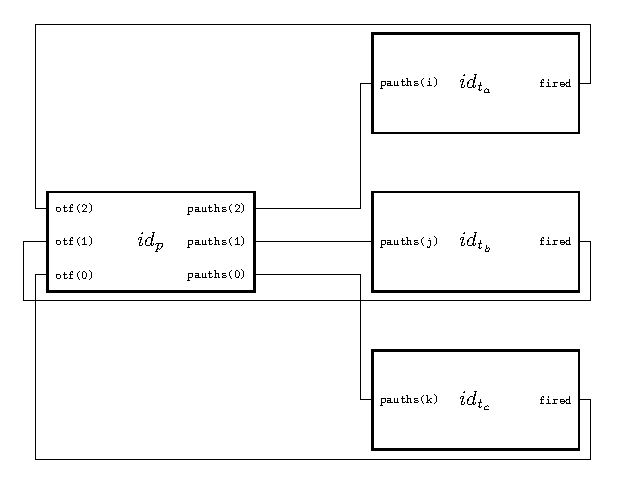
\includegraphics[keepaspectratio, width=.7\textwidth]{Figures/Proof/ordered-indexes}
  \caption[Connection between the \texttt{priority\_authorizations},
  \texttt{output\_transitions\_fired} and \texttt{fired} ports of a
  PCI and 3 TCIs.]{Connection between the
    \texttt{priority\_authorizations} output port of PCI $id_p$ and
    the \texttt{priority\_authorizations} input port of TCIs
    $id_{t_a}$, $id_{t_b}$ and $id_{t_c}$, and between the
    \texttt{output\_transitions\_fired} input port of $id_p$ and the
    \texttt{fired} ports of $id_{t_a}$, $id_{t_b}$ and
    $id_{t_c}$. \texttt{pauths} stands for
    \texttt{priority\_authorizations} and \texttt{otf} stands for
    \texttt{output\_transitions\_fired}.}
  \label{fig:ordered-indexes}
\end{figure}

In Figure~\ref{fig:ordered-indexes}, the indexes in the interface of
$id_p$ respect the priority order of the output transitions. The index
increases as the priority level of the connected TCI decreases. Thus,
$id_{t_c}$ is connected to index 0 as transition $t_c$ is the
top-priority transition in the output transitions of $p$, $id_{t_b}$
is connected to index 1 as $t_c\succ{}t_b$, etc.\\

\noindent{}As a reminder, the current goal to prove is:\\
\fbox{$\sigma'(id_p)(\texttt{s\_marking})-\mathtt{vsots}\ge\sigma'(id)(\texttt{output\_arcs\_weights})[j]$.}\\

The current goal is the \hvhdl{} implementation of the test that the
residual marking in place $p$ enables transition $t$. At the beginning
of the proof, we assumed that transition $t$ is sensitized by the
residual marking for all its input places, i.e.
$t\in{}Sens(s'.M-\sum\limits_{t_i\in{}Pr(t,s')}pre(t_i))$. By looking
at the definition of the $Sens$ set (see Definition~\ref{def:sens}),
and knowing that a basic arc of weight $\omega$ connects place $p$ to
transition $t$, we can deduce that
$s'.M(p)-\sum\limits_{t_i\in{}Pr(t,s')}pre(p,t_i)\ge\omega$. Now, we
must relate the terms of the latter formula to the terms of the
goal. We can easily show, appealing to
Lemma~\ref{lem:fe-equal-marking}, that $s'.M(p)$ equals
$\sigma'(id_p)(\texttt{s\_marking})$. Then, by construction, and
knowing that TCI $id_t$ is connected to PCI $id_p$ through the index
$j$, we can deduce that the $j$-th element of the
\texttt{output\_arcs\_weights} input port denotes the weight of the
arc between place $p$ and transition $t$, i.e. the natural number
$\omega$. The last thing to show is the equality
between the two sum terms:\\
\noindent{}\fbox{
  \begin{tabular}{c}
$\sum\limits_{t_i\in{}Pr(t,s')}
\begin{cases}
  \omega~\mathtt{if}~pre(p,t_i)=(\omega,\mathtt{basic}) \\
  0~otherwise
\end{cases}$\\
$=$\\
$\sum\limits_{l=0}^{j-1}
\begin{cases}
  \sigma'(id_p)(\texttt{oaw})[l]~\mathtt{if}~\sigma'(id_p)(\texttt{otf})[l]~.~(\sigma'(id_p)(\texttt{oat})[l]=\mathtt{basic})\\
  0~otherwise\\
\end{cases}$\\
  \end{tabular}
}\\

On the upper part of the equality, we have unfolded term
$\sum\limits_{t_i\in{}Pr(t,s')}pre(t_i)$ to its full definition (see
Notation~\ref{not:sum-exprs} in Section~\ref{sec:fired-trans}). On the
lower part is the full definition of the \texttt{vsots} term.  Let us
rewrite the two sum terms in a manner that will come handy to prove
the equality. Let us define the $Pr_p$ set, which is the set of fired
transitions with a higher priority than $t$ that are conflicting with
$t$ through the place $p$:

\begin{center}
  $t_i\in{}Pr_p\equiv{}t_i\succ{}t\land\exists\omega~s.t.~pre(p,t_i)=(\omega,\mathtt{basic})\land{}t_i\in{}Fired(s')$
\end{center}

Let us also define the $IPr_p$ set, which the set of indexes from $0$
to $j-1$ for which the \texttt{otf} port of $id_p$ equals
\texttt{true} at state $\sigma'$ and the \texttt{oat} port of $id_p$
equals \texttt{true} at state $\sigma'$:

\begin{center}
  $l\in{}IPr_p\equiv{}l\in[0,j-1]\land(\sigma'(id_p)(\texttt{oat})[l]=\mathtt{basic})\land{}(\sigma'(id_p)(\texttt{otf})[l]=\mathtt{true})$
\end{center}

\noindent{}We can equivalently rewrite the goal as follows: \fbox{$\sum\limits_{t_i\in{}Pr_p}\mathtt{fst}(pre(p,t_i))=\sum\limits_{l\in{}IPr_p}\sigma'(id_p)(\texttt{oaw})[l]$}\\

In the left sum term, the $pre(p,t_i)$ always returns a couple
$(\omega,\mathtt{basic})$ as $t_i$ verifies that there exists an
$\omega$ such that $pre(p,t_i)=(\omega,\mathtt{basic})$. Thus, the
expression $\mathtt{fst}(pre(p,t_i))$ denotes the first element of the
couple returned by $pre(p,t_i)$, i.e. the weight $\omega$.

Then, to prove the above equality, we must show that there exists a
bijection $\beta$ between $Pr_p$ and $IPr_p$ such that for all
$t_i\in{}Pr_p$, we have
$\mathtt{fst}(pre(p,t_i))=\sigma'(id_p)(\mathtt{oaw})[\beta(t_i)]$.
By property of the transformation function, we know that the order of
the indexes in the \texttt{priority\_authorizations} output port of
$id_p$ reflects the priority order of the conflicting output
transitions of place $p$ (see Figure~\ref{fig:ordered-indexes}). Then,
we can exhibit a bijection $\beta_0$ between the output transitions of
$p$ with a higher priority than $t$ and the indexes $l$ of interval
$[0,j-1]$ verifying $\sigma'(id_p)(\texttt{oat})[l]=basic$. However,
to build a complete bijection $\beta$ from $Pr_p$ to $IPr_p$, we need
to know that for a transition $t_i$ that is a conflicting transition
of place $p$ with a higher priority than $t$, we have
$t_i\in{}Fired(s')\Leftrightarrow\sigma'(id_p)(\texttt{otf})[\beta_0(t_i)]=\mathtt{true}$.
By property of the transformation function, we know that the element
of index $\beta_0(t_i)$ of the \texttt{otf} input port of PCI $id_p$
is in fact connected to the \texttt{fired} output port of TCI
$id_{t_i}$. Thus, what we must assume to build a bijection from $Pr_p$
to $IPr_p$ is
$t_i\in{}Fired(s')\Leftrightarrow\sigma'(id_{t_i})(\texttt{fired})=\mathtt{true}$.
This is exactly the property of equivalence between the set of fired
transitions and the value of the \texttt{fired} output ports that we
are currently trying to prove.

Thus, to carry out the proof, we need a strong hypothesis stating that
the equivalence between the set of fired transitions and the
\texttt{fired} ports holds for all transitions with a higher firing
priority than $t$, thus including the ones that are in conflict with
$t$ through place $p$. Therefore, we must think of a way to build the
set of fired transitions iteratively such that the previous hypothesis
becomes an invariant over the many iterations. The recursive
definition of the set of fired transitions naturally calls for a proof
by structural induction over the set of fired transitions.  As stated
before, the actual definition of the set of fired transitions is very
declarative.  However, we can easily convert it into an algorithm that
will build the set iteratively. The result is
Algorithm~\ref{alg:fired}.

\begin{algorithm}[H]
  \DontPrintSemicolon

  % \SetAlFnt{\fontsize{7}{10}\selectfont}
  
  % \SetAlCapFnt{\fontsize{7}{10}\selectfont}
  % \SetAlCapNameFnt{\fontsize{7}{10}\selectfont}
  % \NoCaptionOfAlgo

  \caption{fired($s$)}
  \label{alg:fired}  
  
  \AlFnt % overriding the new font

  \KwData{An SITPN state $s$}
  \KwResult{Returns the set of fired transitions at state $s$}
  
  $F\leftarrow\emptyset$\;
  $T_s\leftarrow{}T$\;
  
  \BlankLine

  \While{$T_s\neq\emptyset$}{\label{line:fired-while}
    $t\leftarrow$ \texttt{GetTopPriorityTransition($T_s$, $\succ$)}\;\label{line:fired-gettp}
    \lIf{$t\in{}Firable(s)$ \textbf{and} $t\in{}Sens(s.M-\sum\limits_{t_i\in{}Pr(t,F)}pre(t_i))$}{\label{line:fired-test}
      $F\leftarrow{}F\cup{}\{t\}$\;
    }

    $T_s\leftarrow{}T_s\setminus{}\{t\}$\;\label{line:fired-withdraw}
  }

  \Return{$F$}\;
\end{algorithm}

Algorithm~\ref{alg:fired} builds the set of fired transitions at state
$s$ by iterating over the set of transitions $T$. Local variables are
initialized in the two first lines. Variable $F$ carries the set of
fired transitions, which is initially empty. Variable $T_s$ represents
the set of transitions still to be processed; $T_s$ is equal to $T$ at
the beginning of the algorithm. At Line~\ref{line:fired-while}, the
\texttt{while} loop iterates until all transitions of the $T_s$ set
have been elected to be fired or have been discarded. At Line
\ref{line:fired-gettp}, function \texttt{GetTopPriorityTransition}
returns a top-priority transition of $T_s$, i.e. a transition $t$ for
which there exists no transition $t'$ in $T_s$ such that $t'\succ{}t$.
The statement of Line~\ref{line:fired-test} tests if the top-priority
transition $t$ is firable at state $s$ and is sensitized by the
residual marking computed by the expression
$s.M-\sum\limits_{t_i\in{}Pr(t,F)}pre(t_i)$. Here, $Pr(t,F)$ is the
set of transitions with the higher priority than $t$ that are in the
set $F$, i.e.: $Pr(t,F)=\{t_i~\vert~t_i\succ{}t\land{}t_i\in{}F\}$.
We know that the following property holds: all fired transitions with
a higher firing priority than $t$ and that have been elected to be
fired are inside the set $F$. Therefore, $F$ contains all the
transitions necessary to compute the residual marking that is
necessary to elect the transition $t$ as a fired transition; if $t$
passes the test of Line~\ref{line:fired-test} then it joins the set
$F$.  The statement of Line~\ref{line:fired-withdraw} withdraws the
transition $t$ from the set $T_s$ before beginning another
iteration. Because the priority relation $\succ$ is a strict order
over the set of transitions $T$, we can always find a top-priority
transition in $T_s$. Thus, there can be no iteration where $T_s$ is
not decreasing. Thus, the algorithm always terminates and returns the
set of fired transitions at state $s$.

Being more accustomed to handle relations while performing a proof, we
make a relational definition of Algorithm~\ref{alg:fired} through the
definition of the $IsFiredSet$ and the $IsFiredSetAux$ relations given
in Definition~\ref{def:is-frd-set} and
\ref{def:is-frd-set-aux}. Definition~\ref{def:cons-fired} states that
a given transition is fired in relation to the $IsFiredSet$ relation.

\begin{definition}[Fired]
  \label{def:cons-fired}
  A transition $t\in{}T$ is said to be fired at the SITPN state
  $s={<}M,I,reset_t,$ $ex,$ $cond{>}$, iff there exists a subset
  $Fset\subseteq{}T$ such that $IsFiredSet(s,Fset)$ and $t\in{}Fset$.
\end{definition}

\begin{definition}[IsFiredSet]
  \label{def:is-frd-set}
  Given an $sitpn\in{}SITPN$, a SITPN state $s\in{}S(sitpn)$, and a
  subset $Fset\subseteq{}T$, the $IsFiredSet$ relation is defined as follows:\\
  $IsFiredSet(s,Fset)\equiv{}IsFiredSetAux(s,T,\emptyset,Fset)$
\end{definition}

\begin{definition}[IsFiredSetAux]
  \label{def:is-frd-set-aux}
  The $IsFiredSetAux$ relation is defined by the following rules:\\
  \begin{tabular}{@{}l}
    {\fontsize{9}{11}\selectfont\textsc{FSetEmp}} \\
    
    {\begin{prooftree}[template={\inserttext}]        
        \infer0{$IsFiredSetAux(s, \emptyset, F, F)$}
      \end{prooftree}} 
  \end{tabular}
  \begin{tabular}{@{}l}
    {\fontsize{9}{11}\selectfont\textsc{FSetFired}} \\
    
    {\begin{prooftree}[template={\inserttext}]

        \hypo{$t\in{}Firable(s)$}
        \infer[no rule]1{$t\in{}Sens(s.M-\sum\limits_{t_i\in{}Pr(t,F)}pre(t_i))$}
        \infer[no rule]1{$IsFiredSetAux(s, T_s, F\cup\{t\}, Fset)$}
        \infer1[
        \begin{tabular}{@{}l}
          $\nexists{}t'\in{}T_s~s.t.~t'\succ{}t$ \\
          $Pr(t,F)=\{t'~\vert~t'\succ{}t\land{}t'\in{}F\}$ \\
        \end{tabular}
        ]{$IsFiredSetAux(s, T_s\cup\{t\}, F, Fset)$}
      \end{prooftree}} 
  \end{tabular}
  
  \begin{tabular}{@{}l}
    {\fontsize{9}{11}\selectfont\textsc{FSetNotFirable}} \\    
    {\begin{prooftree}[template={\inserttext}]
        \hypo{$t\notin{}Firable(s)$}
        \infer[no rule]1{$IsFiredSetAux(s, T_s, F, Fset)$}
        \infer1[
        \begin{tabular}{@{}l}
          $\nexists{}t'\in{}T_s~s.t.~t'\succ{}t$ \\
        \end{tabular}
        ]{$IsFiredSetAux(s, T_s\cup\{t\}, F, Fset)$}
      \end{prooftree}} 
  \end{tabular}
  
  \begin{tabular}{@{}l}
    {\fontsize{9}{11}\selectfont\textsc{FSetNotSens}} \\
    {\begin{prooftree}[template={\inserttext}]
        \hypo{$t\notin{}Sens(s.M-\sum\limits_{t_i\in{}Pr(t,F)}pre(t_i))$}
        \infer[no rule]1{$IsFiredSetAux(s, T_s, F, Fset)$}
        \infer1[
        \begin{tabular}{@{}l}
          $\nexists{}t'\in{}T_s~s.t.~t'\succ{}t$ \\
          $Pr(t,F)=\{t'~\vert~t'\succ{}t\land{}t'\in{}F\}$ \\
        \end{tabular}
        ]{$IsFiredSetAux(s, T_s\cup\{t\}, F, Fset)$}
      \end{prooftree}} 
  \end{tabular}
\end{definition}

We are now satisfied with the definition of the set of fired
transitions provided by the $IsFiredSet$ relation and the
$IsFiredSetAux$ relation. Therefore, we give a new expression to
Lemma~\ref{lem:fe-equal-fired} by using the $IsFiredSet$ relation to
qualify the set of fired transitions instead of using the first
declarative definition. The result is
Lemma~\ref{lem:fe-equal-fset}.




The full formal proof of Lemma~\ref{lem:fe-equal-fset} is given in
Section~\ref{sec:falling-edge} of
Appendix~\ref{app:sem-preserv-proof}.  The inductive definition of the
$IsFiredSetAux$ relation permits us to express the hypothesis that we
lacked to perform the proof of Lemma~\ref{lem:fe-equal-fired}. The
hypothesis saying that for a given transition $t$, the ``fired''
equivalence holds for all transitions with a higher firing
priority. This is stated in the ``extra'' hypothesis used in
Lemma~\ref{lem:fe-equal-fset-aux}.

\subsection{A report on a bug detection}
\label{sec:bug-detection}

In the previous section, we showed the equivalence between fired
transitions and \texttt{fired} port values at the end of the falling
edge phase. In a previous definition of the SITPN state, preceding the
bug detection, the set of fired transitions was a member of the SITPN
state record. For a given $sitpn\in{}SITPN$, we defined an SITPN state
$s$ by the record $s={<}Fired,M,I,cond,ex{>}$ where $Fired$ was the
set of fired transitions.  The $Fired$ set was involved in the
computation of time counter values during the falling edge
phase. Thus, we needed the proof that the equivalence between the set
of fired transitions and the value of the \texttt{fired} ports was
effective at the beginning of the falling edge phase. In the previous
SITPN semantics, the set of fired transitions stayed the same during
the rising edge phase. Therefore, between two SITPN states $s, s'$
verifying the rising edge state transition relation, i.e.
$s\xrightarrow{\uparrow}s'$, we had $s.Fired=s'.Fired$. However, we
showed that it wasn't the case on the \hvhdl{} side, i.e. the values
of the \texttt{fired} ports in TCIs would not stay the same during the
rising edge phase. Thus, the equivalence fired transitions and
\texttt{fired} port values at the end of the falling edge phase. The
consequence was a divergence between the value of time counters and
the value of the \texttt{s\_time\_counter} signals, both computed
during the falling edge phase. Figure~\ref{fig:diverg-tc} shows a case
of divergence between time counters and \texttt{s\_time\_counter}
signals values in the course of an execution.

\begin{figure}[H]
  \centering
  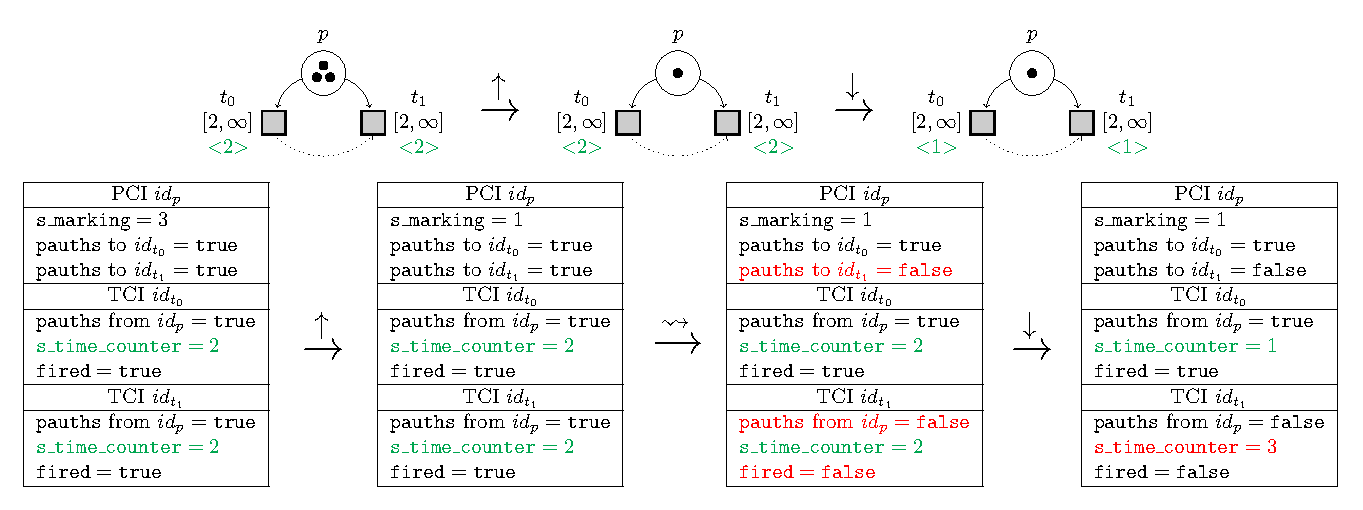
\includegraphics[keepaspectratio,width=\textwidth]{Figures/Proof/diverg-tc}
  \caption[Bug Detection in the place and transition designs.]{Bug detection: divergence between the value of time counters and the value of the $\mathtt{s\_time\_counter}$ signals due to the loss of the firing status information during the stabilization phase; the value of time counters and of the $\mathtt{s\_time\_counter}$ signals are in green; the value of diverging signals are in red.}
  \label{fig:diverg-tc}
\end{figure}

In Figure~\ref{fig:diverg-tc}, during the stabilization phase coming
right after the rising edge of the clock, the value of the
\texttt{fired} port of TCI $id_{t_1}$ passes to \texttt{false}. After
the update of the \texttt{s\_marking} signal value during the rising
edge phase, PCI $id_p$ computes new priority authorizations for its
output TCIs. As the marking is only sufficient to fire transition
$t_0$ but not transition $t_1$, PCI $id_p$ indicates to TCI $id_{t_1}$
that it no longer has the authorization to fire. Consequently, through
the connection of \texttt{priority\_authorizations} ports, the value
of the \texttt{fired} port of $id_{t_1}$ is set to \texttt{false}.
Following the rules of the SITPN semantics, on the next falling edge,
the value of time counters must be reset for transition $t_0$ and
$t_1$, because both were fired at the previous rising edge. As a part
of the behavior of a TCI, the \texttt{time\_counter} process, executed
at the falling edge of the clock, resets the value of the
\texttt{s\_time\_counter} signal given that the value of the
\texttt{fired} port is true. Thus, as the value of the \texttt{fired}
port of TCI $id_{t_1}$ is false at the falling edge, the
\texttt{time\_counter} process increments the value of the
\texttt{s\_time\_counter} signal instead of resetting its value. The
consequence is a divergence between the value of the time counter of
transition $t_1$ and the value of the \texttt{s\_time\_counter} signal
in TCI $id_{t_1}$.

As demonstrated above, the \texttt{time\_counter} process can not rely
on the value of the \texttt{fired} ports to determine if the value of
the \texttt{s\_time\_counter} signal must be reset or not. We proved
that there is an equivalence between the fired transitions and the
value of the \texttt{fired} ports at the end of a falling edge
phase. We need a way to memorize the value of \texttt{fired} ports at
the moment where the equivalence holds (i.e. at the end of the falling
edge phase) so that the \texttt{time\_counter} process can use this
information to reset the \texttt{s\_time\_counter} signal. To do so,
we have modified the SITPN semantics and the behavior of the
transition design. In the actual version of the SITPN semantics, if a
transition is fired at the beginning of the rising edge phase then a
reset order is sent to the transition. As a consequence, the time
counter associated to this transition will be reset at the next
falling edge. In the actual version of the transition design behavior,
the value of the \texttt{fired} port is involved in the computation of
the \texttt{s\_reinit\_time\_counter} signal; the
\texttt{s\_reinit\_time\_counter} signal value follows the value of
the reset order assigned to a given transition. Thus, as the
equivalence between reset orders and the value of the
\texttt{s\_reinit\_time\_counter} signal holds at the beginning of the
falling edge phase, the \texttt{time\_counter} process can rely on the
value of the \texttt{s\_reinit\_time\_counter} signal to reset the
value of the \texttt{s\_time\_counter} signal. As a consequence, the
set of fired transitions is no longer involved in the SITPN semantics
premises of the falling edge phase. Therefore, we chose to withdraw
the $Fired$ set from the definition of the SITPN state record. We
opted for an intentional definition of the set of fired transitions at
given SITPN state (i.e., Definition~\ref{def:fired}). After these
changes, we were able to prove that there were no more divergence
between the time counters and the value of the
\texttt{s\_time\_counter} signals in the course of the execution (see
Lemmas~\ref{lem:re-equal-tc}, p.~\pageref{lem:re-equal-tc}, and
\ref{lem:fe-equal-tc}, p.~\pageref{lem:fe-equal-tc}, about the
equivalence of time counters).

%%% Local Variables:
%%% mode: latex
%%% TeX-master: "../../main"
%%% End:
